\documentclass[11pt, fleqn]{beamer}\usepackage[]{graphicx}\usepackage[]{color}
% maxwidth is the original width if it is less than linewidth
% otherwise use linewidth (to make sure the graphics do not exceed the margin)
\makeatletter
\def\maxwidth{ %
  \ifdim\Gin@nat@width>\linewidth
    \linewidth
  \else
    \Gin@nat@width
  \fi
}
\makeatother

\definecolor{fgcolor}{rgb}{0.345, 0.345, 0.345}
\newcommand{\hlnum}[1]{\textcolor[rgb]{0.686,0.059,0.569}{#1}}%
\newcommand{\hlstr}[1]{\textcolor[rgb]{0.192,0.494,0.8}{#1}}%
\newcommand{\hlcom}[1]{\textcolor[rgb]{0.678,0.584,0.686}{\textit{#1}}}%
\newcommand{\hlopt}[1]{\textcolor[rgb]{0,0,0}{#1}}%
\newcommand{\hlstd}[1]{\textcolor[rgb]{0.345,0.345,0.345}{#1}}%
\newcommand{\hlkwa}[1]{\textcolor[rgb]{0.161,0.373,0.58}{\textbf{#1}}}%
\newcommand{\hlkwb}[1]{\textcolor[rgb]{0.69,0.353,0.396}{#1}}%
\newcommand{\hlkwc}[1]{\textcolor[rgb]{0.333,0.667,0.333}{#1}}%
\newcommand{\hlkwd}[1]{\textcolor[rgb]{0.737,0.353,0.396}{\textbf{#1}}}%
\let\hlipl\hlkwb

\usepackage{framed}
\makeatletter
\newenvironment{kframe}{%
 \def\at@end@of@kframe{}%
 \ifinner\ifhmode%
  \def\at@end@of@kframe{\end{minipage}}%
  \begin{minipage}{\columnwidth}%
 \fi\fi%
 \def\FrameCommand##1{\hskip\@totalleftmargin \hskip-\fboxsep
 \colorbox{shadecolor}{##1}\hskip-\fboxsep
     % There is no \\@totalrightmargin, so:
     \hskip-\linewidth \hskip-\@totalleftmargin \hskip\columnwidth}%
 \MakeFramed {\advance\hsize-\width
   \@totalleftmargin\z@ \linewidth\hsize
   \@setminipage}}%
 {\par\unskip\endMakeFramed%
 \at@end@of@kframe}
\makeatother

\definecolor{shadecolor}{rgb}{.97, .97, .97}
\definecolor{messagecolor}{rgb}{0, 0, 0}
\definecolor{warningcolor}{rgb}{1, 0, 1}
\definecolor{errorcolor}{rgb}{1, 0, 0}
\newenvironment{knitrout}{}{} % an empty environment to be redefined in TeX

\usepackage{alltt}
\usepackage{amsmath}
\usepackage{amssymb}
\usepackage{geometry}
\usepackage{graphicx}
\usepackage{url}
\IfFileExists{upquote.sty}{\usepackage{upquote}}{}
\begin{document}

\begin{frame}
\large
Lecture 12:\\
Simple Linear Regression\\
STAT 310, Spring 2021
\end{frame}

%---------------------------------------------
\begin{frame}{Scatterplots}
\begin{itemize}
\item A scatterplot a graphical display used to study the relationship between two numerical variables $x$ and $y$.  
\vspace{5pt}
\item Data displayed on a scatterplot are collected in pairs:
$$(x_1, y_1), (x_2, y_2), \cdots, (x_n, y_n)$$
where $n$ denotes the total number of cases or pairs.
\vspace{5pt}
% \item $y$ is commonly called the \textbf{response variable} and $x$ the \textbf{explanatory variable}.
\vspace{5pt}
\item A scatterplot provides insight into how two variables are related. 
\end{itemize}
\end{frame}

%---------------------------------------------
\begin{frame}{Example}
A scatterplot showing the association between first year college GPA and high school GPA for a random sample of 150 students.
\begin{figure}
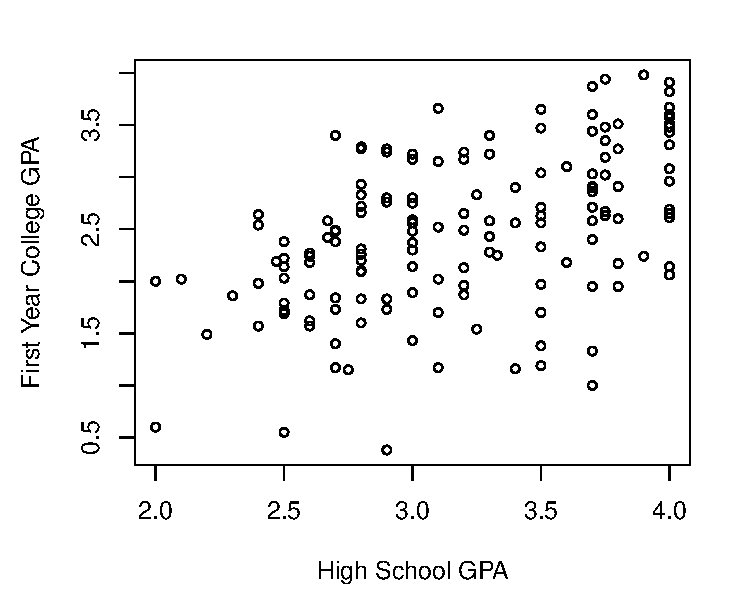
\includegraphics[scale=0.5]{figure/gpa_scatter1.pdf}
\end{figure}
\end{frame}

%---------------------------------------------
\begin{frame}{Types of Relationships Between Variables}
\begin{itemize}
\item Two variables are said to be \textbf{associated} if the scatterplot shows a discernible pattern or trend.
\vspace{5pt}
\item An association is \textbf{positive} if $y$ increases as $x$ increases.
\vspace{5pt}
\item An association is \textbf{negative} if $y$ decreases as $x$ increases.
\vspace{5pt}
\item An association is \textbf{linear} if the scatterplot between $x$ and $y$ has a linear trend; otherwise, the association is called \textbf{nonlinear}. 
\end{itemize}
\end{frame}

%---------------------------------------------
\begin{frame}
\centering
\begin{figure}
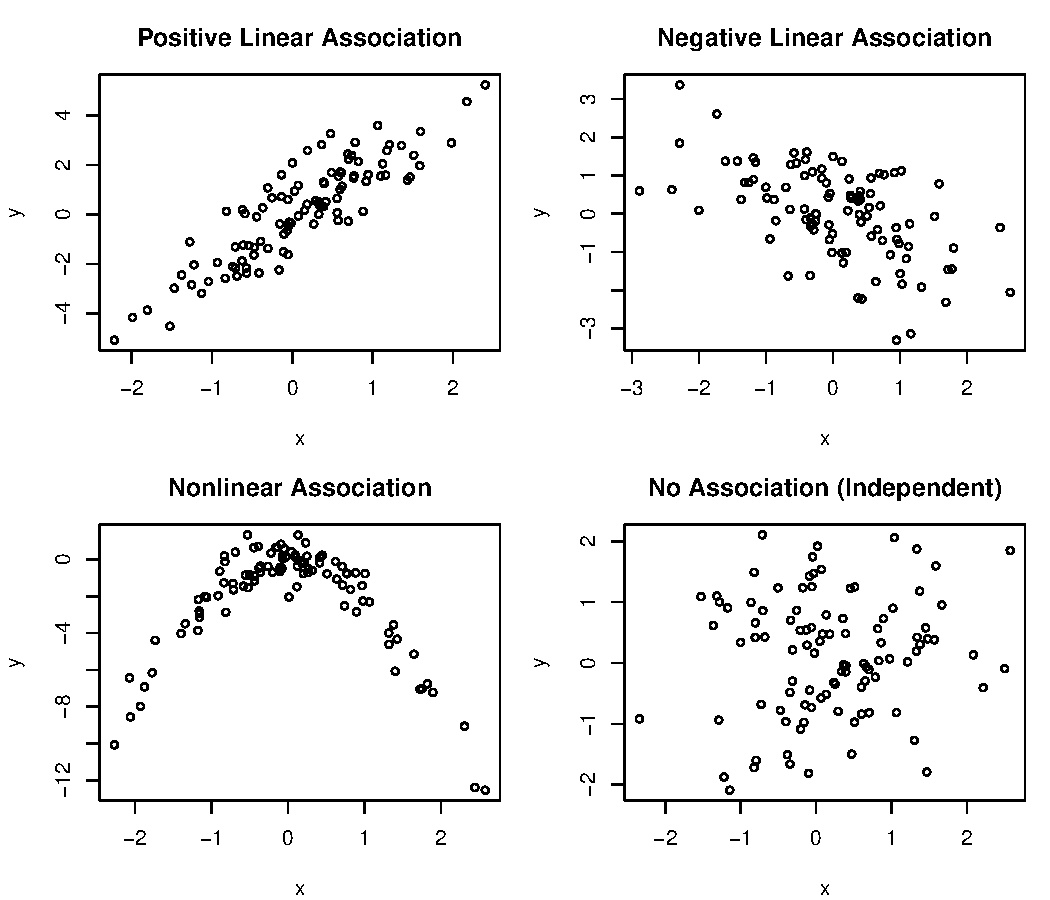
\includegraphics[scale=0.5]{figure/associations.pdf}
\end{figure}
\end{frame}

%---------------------------------------------
\begin{frame}{Correlation Coefficient}
The \textbf{correlation coefficient}, denoted by $r$, is a number between -1 and 1 that describes the strength of the linear association between two variables.
\begin{figure}
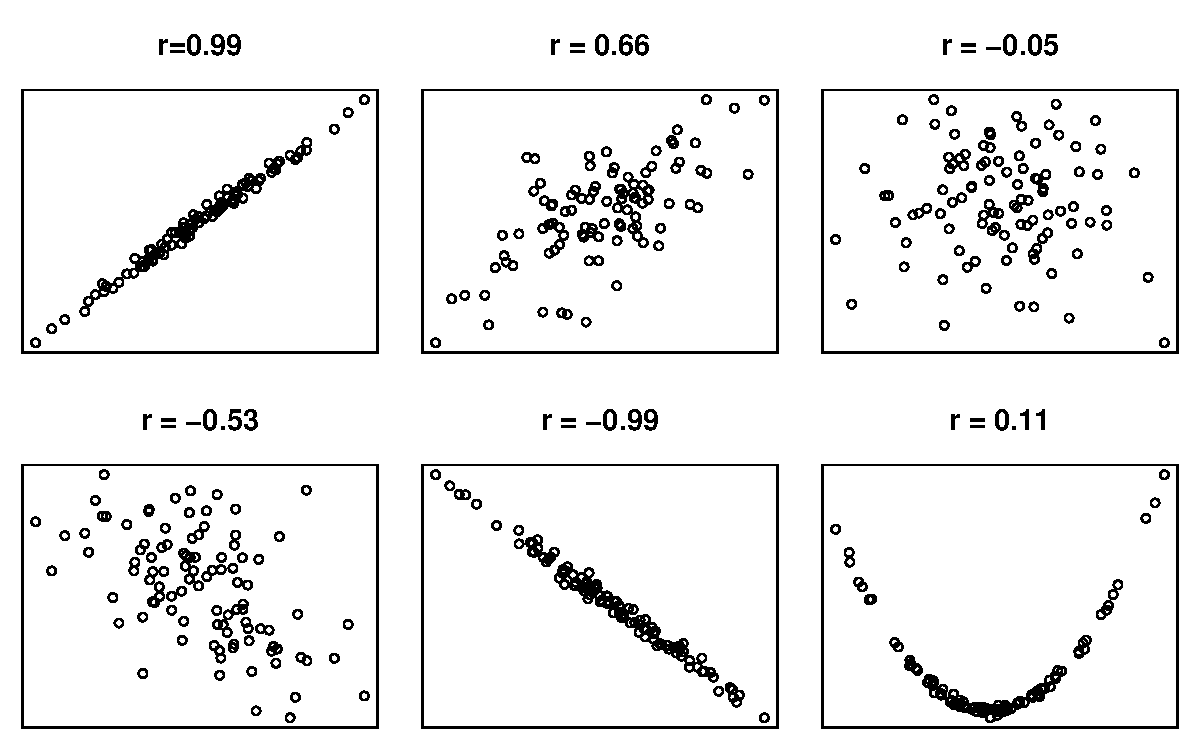
\includegraphics[scale=0.4]{figure/correlations.pdf}
\end{figure}
\end{frame}

%---------------------------------------------
\begin{frame}{Correlation Coefficient}
\begin{itemize}
\item $r \approx 1$ when there is a strong positive linear association between the variables.
\vspace{5pt}
\item $r \approx -1$ when there is a strong negative linear association between the variables.
\vspace{5pt}
\item $r \approx 0$ when there is no association between the variables (i.e., independent).
\vspace{5pt}
\item The correlation coefficient is only useful for evaluating the linear association between two variables.  It is not a useful measure for nonlinear relationships.
\end{itemize}
\end{frame}

%---------------------------------------------
\begin{frame}{Correlation Coefficient}
Formally, the correlation can be calculated using the following formula.  The formula is rather complex, so we use software packages such as R to do the calculations for us.\\ 

\begin{align*}
r = \frac{1}{n-1} \sum_{i=1}^n \left(\frac{x_i - \bar{x}}{s_x} \right) \left( \frac{y_i - \bar{y}}{s_y} \right)
\end{align*}
\begin{itemize}
\item $\bar{x}$ and $\bar{y}$ are the sample means
\item $s_x$ and $s_y$ are the sample standard deviations
\end{itemize}
\end{frame}

%---------------------------------------------
\begin{frame}{Example}
Match each correlation to the corresponding scatterplot.
\begin{enumerate}[(a)]
\item $r = -0.63$
\item $r = 0.85$
\item $r = 0.19$
\item $r = 0.95$
\end{enumerate}
\begin{figure}
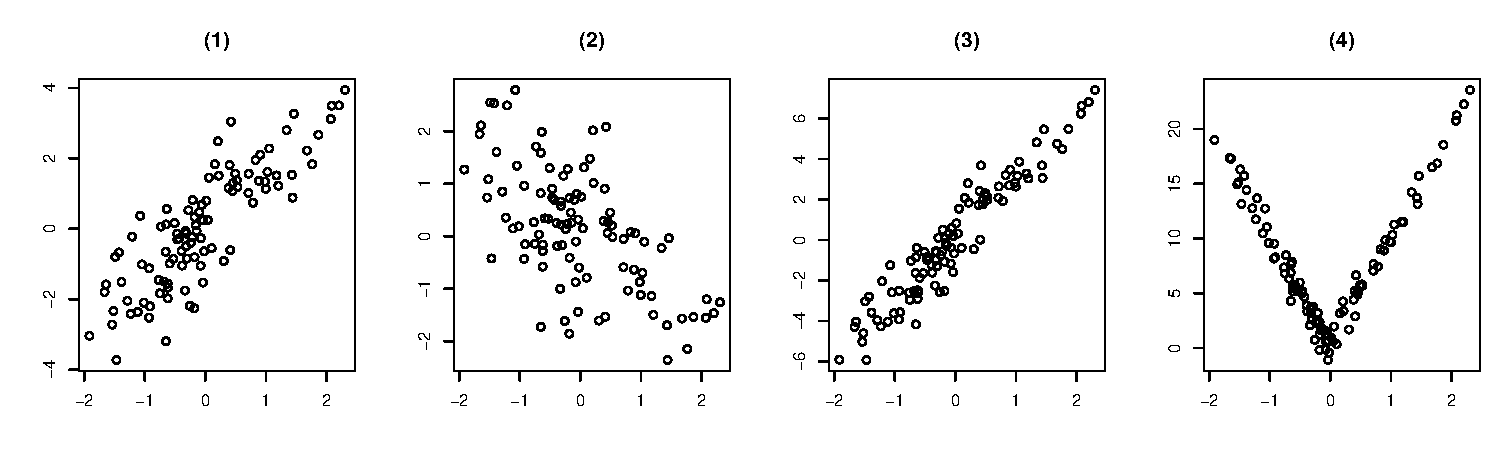
\includegraphics[scale=0.4]{figure/cor_prob.pdf}
\end{figure}
\end{frame}

%---------------------------------------------
\begin{frame}{Simple Linear Regression}
\begin{itemize}
\item \textbf{Simple linear regression} is a method for fitting a straight line to data that show a linear trend when displayed on a scatterplot.
\item The method is useful for making predictions and explaining the relationship between two numerical variables.
%\item In the plot below we see that the points do not fall directly on the line.  Instead, we see a cloud of points that vary around the straight line.
\end{itemize}
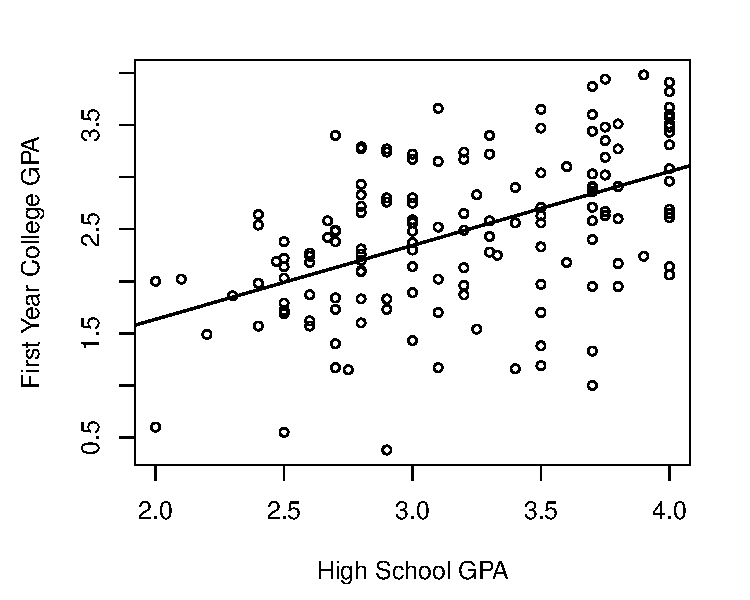
\includegraphics[scale=0.5]{figure/gpa_scatter_line.pdf}
\end{frame}

%---------------------------------------------
\begin{frame}{Simple Linear Regression}
A \textbf{simple linear regression model} expresses the relationship between two variables, $x$ and $y$, as a straight line with some error:
$$y = \beta_0 + \beta_1 x + \epsilon$$
\begin{itemize}
\item $y$ is called the \textbf{response} variable
\item $x$ is called the \textbf{explanatory} or \textbf{predictor} variable.
\item $\beta_0$ is the \textbf{intercept} parameter
\item $\beta_1$ is the \textbf{slope} parameter
\item $\epsilon$ is called the \textbf{random error} term.  It captures the variability in the points around the line.
\end{itemize}
\end{frame}
% which of the following is the most likely value for the correlation between 

%---------------------------------------------
\begin{frame}{Fitted Values and Residuals}
\begin{itemize}
\item The line that we estimate, or fit to the data in the scatterplot, is written as
$$\hat{y} = \hat{\beta}_0 + \hat{\beta}_1 x$$
% where $\hat{\beta}_0$ and $\hat{\beta}_1$ denote the estimates of the regression parameters $\beta_0$ and $\beta_1$.

\item The fitted (or predicted) value for the $i^{th}$ observation $(x_i, y_i)$:
$$\hat{y}_i = \hat{\beta}_0 + \hat{\beta}_1 x_i$$

\item The \textbf{residual} for the $i^{th}$ observation is the difference between the observed value ($y_i$) and the predicted value ($\hat{y}_i$):\\
$$\hat{e}_i = y_i - \hat{y}_i = y_i - (\hat{\beta}_0 + \hat{\beta}_1 x_i)$$
\end{itemize}
\end{frame}

%---------------------------------------------
\begin{frame}
\begin{figure}
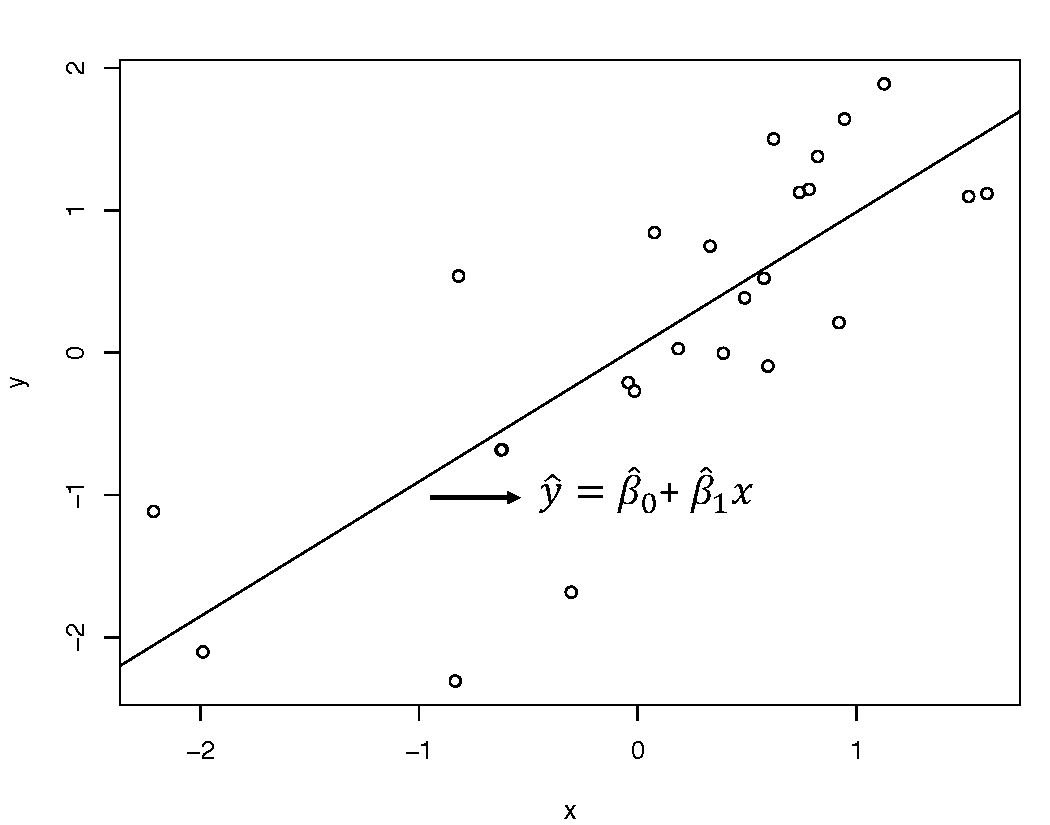
\includegraphics[scale=0.5]{figure/scatter2_2.pdf}
\end{figure}
\end{frame}

%---------------------------------------------
\begin{frame}
\begin{figure}
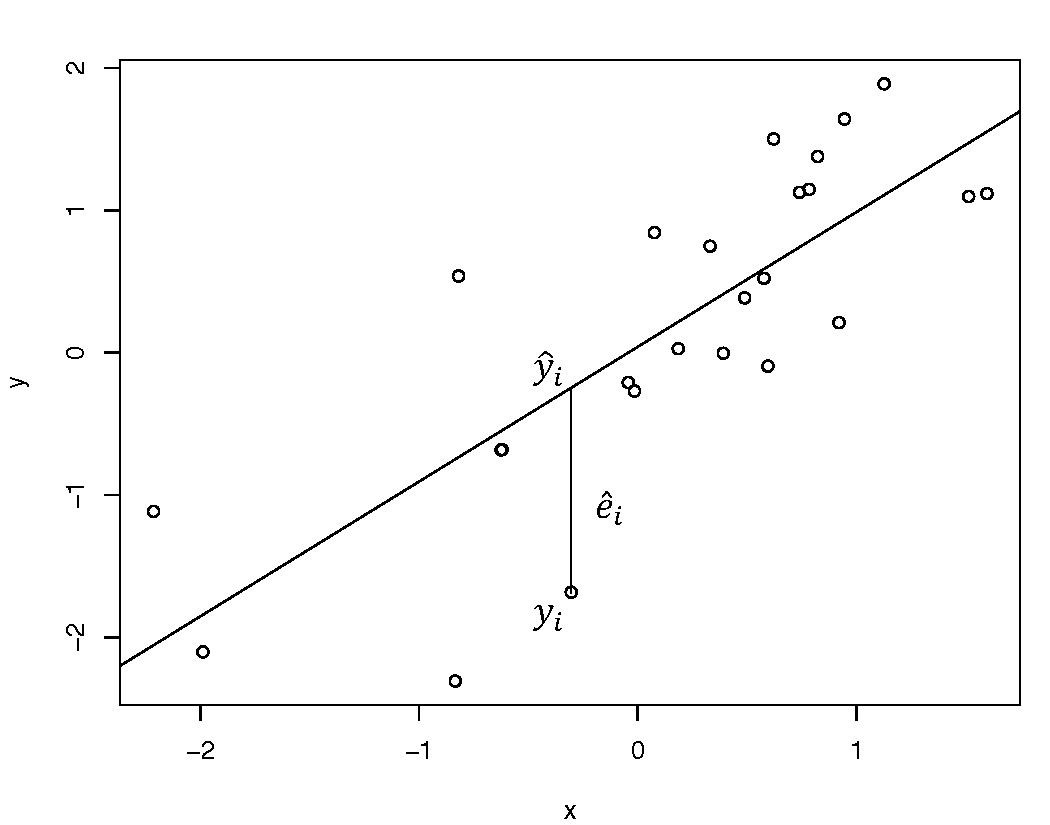
\includegraphics[scale=0.5]{figure/scatter3_2.pdf}
\end{figure}
\end{frame}

%---------------------------------------------
\begin{frame}
\begin{figure}
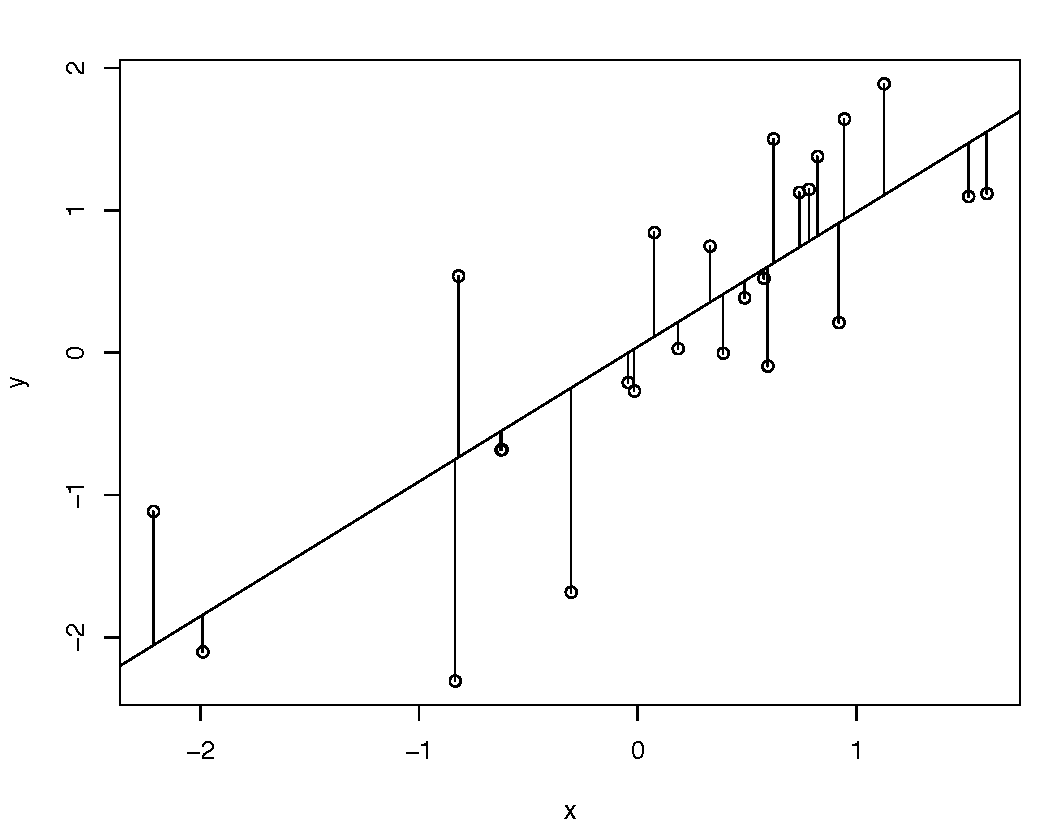
\includegraphics[scale=0.5]{figure/scatter4_2.pdf}
\end{figure}
\end{frame}

%---------------------------------------------
\begin{frame}{Sum of Squared Residuals}
\begin{itemize}
\item Intuitively, a line that fits the data well has small residuals.
\vspace{5pt}
\item The \textbf{least squares line} minimizes the \textbf{sum of squared residuals}:
$$RSS = \sum_{i=1}^n \hat{e}_i^2 = \sum_{i=1}^n (y_i - \hat{\beta}_0 - \hat{\beta}_1 x_i)^2$$
\vspace{5pt}
\item That is, out of all possible lines we could draw on the scatterplot, the least squares line is the ``best fit" since it has the smallest sum of squared residuals.
\end{itemize}
\vspace{1.5cm}
% write out summary
\end{frame}

%---------------------------------------------
\begin{frame}{Least Squares Estimates}
It can be shown (using calculus) that the estimates of the intercept and slope that minimize the sum of squared residuals are given by the following formulas:
\begin{align*}
\hat{\beta}_0 &= \bar{y} - \hat{\beta}_1 \bar{x}\\
\hat{\beta}_1 &= r \frac{s_y}{s_x}
\end{align*}
where $r$ is the correlation coefficient, previously discussed.  Note that the equation for the intercept guarantees the least squares line passes through the point $(\bar{x}, \bar{y})$.
\end{frame}

%---------------------------------------------
\begin{frame}{Example}
\vspace{-0.5cm}
The least squares regression line in the scatterplot is given by:
$$\hat{y} = 0.217 + 0.709\,x$$
Suppose a student graduates high school with a 3.0 GPA.  What is the predicted first year college GPA for this student?
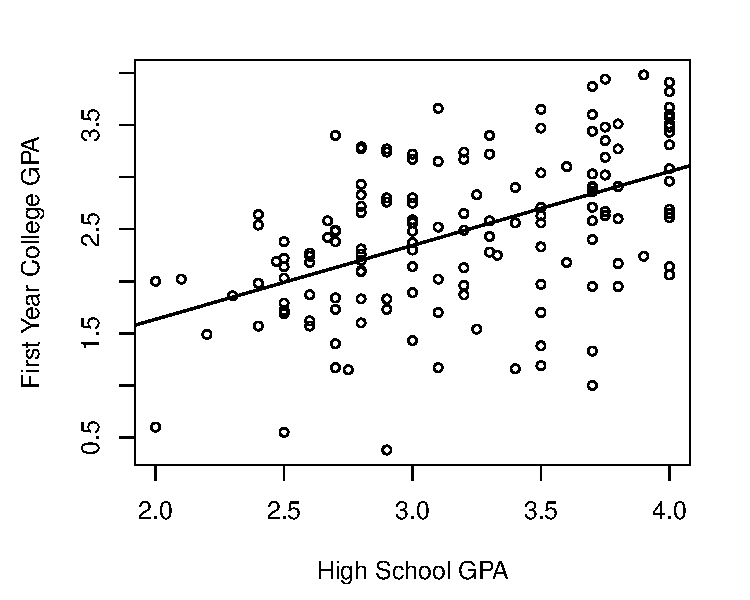
\includegraphics[scale=0.4]{figure/gpa_scatter_line.pdf}
\end{frame}

%---------------------------------------------
\begin{frame}{Example}
\vspace{-0.5cm}
The least squares regression line in the scatterplot is given by:
$$\hat{y} = 0.217 + 0.709\,x$$
Calculate the residual (show in red) for a student, in this data set, that had a 2.7 high school GPA and a 3.4 college GPA.
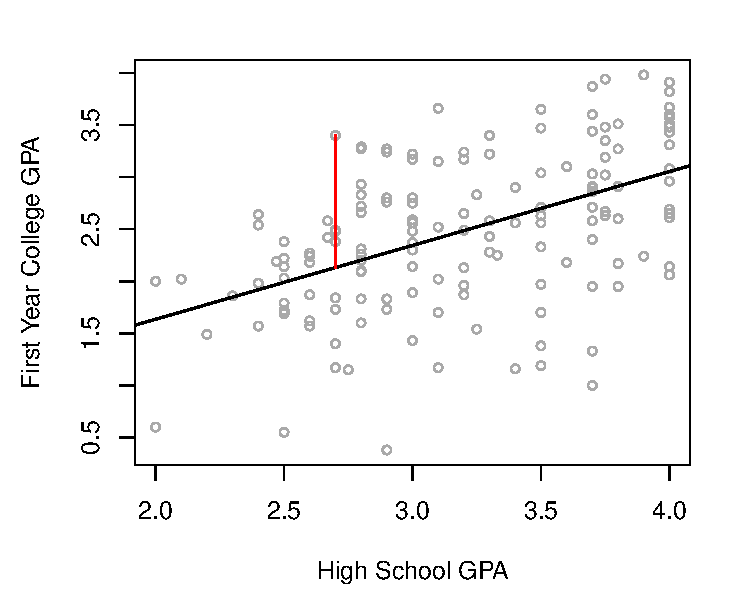
\includegraphics[scale=0.4]{figure/gpa_scatter_resid.pdf}
\end{frame}
% 1.2687

%---------------------------------------------
\begin{frame}{Example}
Use the summary statistics in the table below to manually calculate the slope and intercept of the least squares line.\\

\begin{table}
\begin{tabular}{lll}
\hline
 & HS GPA (x) & FY College GPA (y)\\
\hline
Mean & $\bar{x} = 3.196$ & $\bar{y}=2.48$\\
SD & $s_x = 0.534$ & $s_y=0.753$\\
\hline
& correlation & $r=0.502$\\
\hline
\end{tabular}
\end{table}

\vspace{3.5cm}
\end{frame}

%------------------------------------------------------
\begin{frame}{Interpreting Coefficients}
\vspace{-2.5cm}
\begin{itemize}
\item \textbf{Slope}: an increase in the explanatory variable ($x$) by one unit is associated with a change of $\hat{\beta}_1$ in the predicted response ($\hat{y}$).
\vspace{10pt}
\item \textbf{Intercept}: the prediction for the response variable ($\hat{y}$) when the value for the explanatory variable is zero ($x=0$).  It may not make sense to try to interpret the intercept depending on the application.
\end{itemize}
\end{frame}

%------------------------------------------------------
\begin{frame}{Interpreting Coefficients}
The least squares regression line for predicting first year college GPA (y) from high school GPA (x) is given by:
$$\hat{y} = 0.217 + 0.709\,x$$
Interpret the slope and intercept of this model.
\vspace{4.5cm}
\end{frame}

%------------------------------------------------------
\begin{frame}{Coefficient of Determination ($R^2$)}
\begin{itemize}
\item The coefficient of determination ($R^2$) is a measure of how well the linear regression model fits the data.
\vspace{5pt}
\item The $R^2$ can be computed as the correlation coefficient $r$ squared.
\vspace{5pt}
\item $R^2$ can be interpreted as the proportion of variability in the response variable $y$ that is explained by $x$.
\vspace{5pt}
\item $R^2$ is always between 0 and 1; the closer $R^2$ is to 1, the better the linear regression model fits the data.
\end{itemize}
\end{frame}

%------------------------------------------------------
\begin{frame}{Coefficient of Determination ($R^2$)}
\begin{itemize}
\item Going back to the example, the correlation between high school GPA and first year college GPA is 0.502.
\vspace{5pt}
\item So $R^2 = (0.502)^2 = 0.252$.
\vspace{5pt}
\item This tells us that about 25\% of the variability in first year college GPA (y) can be explained by high school GPA (x).
\end{itemize}
\end{frame}

\end{document}
